\chapter{Stand der Technik}

\section{Agile Softwareentwicklung}

Diese Arbeit dreht sich um agile Teams, deshalb ist es essentiell, zu verstehen, was der Gedanke hinter dem agilen Entwicklungsansatz ist.
Seinen Ursprung hat das Ganze, als sich 2001 ein paar schlaue Köpfe zusammengeschlossen haben und das sogenannte agile Manifest, sowie die agilen Prinzipien aufgestellt haben.
Ziel war es, eine Alternative zu den bisherigen, schwergewichtigen und von Dokumentation getriebenen Softwareentwicklungs-Methodologien zu finden.

\subsection{Agiles Manifest}

Das agile Manifest ist er Grundbaustein aller agilen Vorgehensmodelle:

\begin{quote}Wir erschließen bessere Wege, Software zu entwickeln,
indem wir es selbst tun und anderen dabei helfen.
Durch diese Tätigkeit haben wir diese Werte zu schätzen gelernt: \newline
\begin{center}
Individuen und Interaktionen mehr als Prozesse und Werkzeuge \newline
Funktionierende Software mehr als umfassende Dokumentation \newline
Zusammenarbeit mit dem Kunden mehr als Vertragsverhandlungen \newline
Reagieren auf Veränderung mehr als das Befolgen eines Plans \newline
\end{center}
Das heißt, obwohl wir die Werte auf der rechten Seite wichtig finden,
schätzen wir die Werte auf der linken Seite höher ein.\end{quote}\cite{agile_manifest}

\subsection{Agile Prinzipien}

Die agile Softwareentwicklung folgt diesen zwölf Prinzipien:

\begin{quote}Unsere höchste Priorität ist es, den Kunden durch frühe und kontinuierliche Auslieferung wertvoller Software zufrieden zu stellen.

Heisse Anforderungsänderungen selbst spät in der Entwicklung willkommen. Agile Prozesse nutzen Veränderungen zum Wettbewerbsvorteil des Kunden.

Liefere funktionierende Software regelmäßig innerhalb weniger Wochen oder Monate und bevorzuge dabei die kürzere Zeitspanne.

Fachexperten und Entwickler müssen während des Projektes täglich zusammenarbeiten.

Errichte Projekte rund um motivierte Individuen. Gib ihnen das Umfeld und die Unterstützung, die sie benötigen und vertraue darauf, dass sie die Aufgabe erledigen.

Die effizienteste und effektivste Methode, Informationen an und innerhalb eines Entwicklungsteams zu übermitteln, ist im Gespräch von Angesicht zu Angesicht.

Funktionierende Software ist das wichtigste Fortschrittsmaß.

Agile Prozesse fördern nachhaltige Entwicklung. Die Auftraggeber, Entwickler und Benutzer sollten ein gleichmäßiges Tempo auf unbegrenzte Zeit halten können.

Ständiges Augenmerk auf technische Exzellenz und gutes Design fördert Agilität.

Einfachheit -\phantom{}- die Kunst, die Menge nicht getaner Arbeit zu maximieren -\phantom{}- ist essenziell.

Die besten Architekturen, Anforderungen und Entwürfe entstehen durch selbstorganisierte Teams.

In regelmäßigen Abständen reflektiert das Team, wie es effektiver werden kann und passt sein Verhalten entsprechend an.\end{quote}\cite{agile_principles}

\newpage
\section{Scrum~\footcite[vgl.][S.13ff]{scrum_kurz_gut_2013}}

Das Scrum Framework ist eine solche agile Softwareentwicklungs-Methodologie. 
Scrum basiert auf Empirismus, also der Theorie, dass Wissen aus Erfahrung erlangt wird und Entscheidungen auf Basis dieses Wissens getroffen werden. 
Die drei Grundsäulen einer solchen empirischen Prozesskontrolle sind:

\begin{description}
  \item[Transparenz] \hfill \\ Signifikante Aspekte des Prozesses müssen für alle sichtbar sein.
  \item[Inspektion] \hfill \\ Artefakte müssen regelmäßig inspiziert werden, aber dieser Vorgang darf der Arbeit selbst nicht im Weg stehen.
  \item[Adaption] \hfill \\ Weicht ein oder mehrere Aspekte eines Prozesses von seinen akzeptablen Limits ab, muss dieser so früh wie möglich angepasst werden.
\end{description}

\begin{savenotes}
  \begin{figure}[H] 
    \centering
    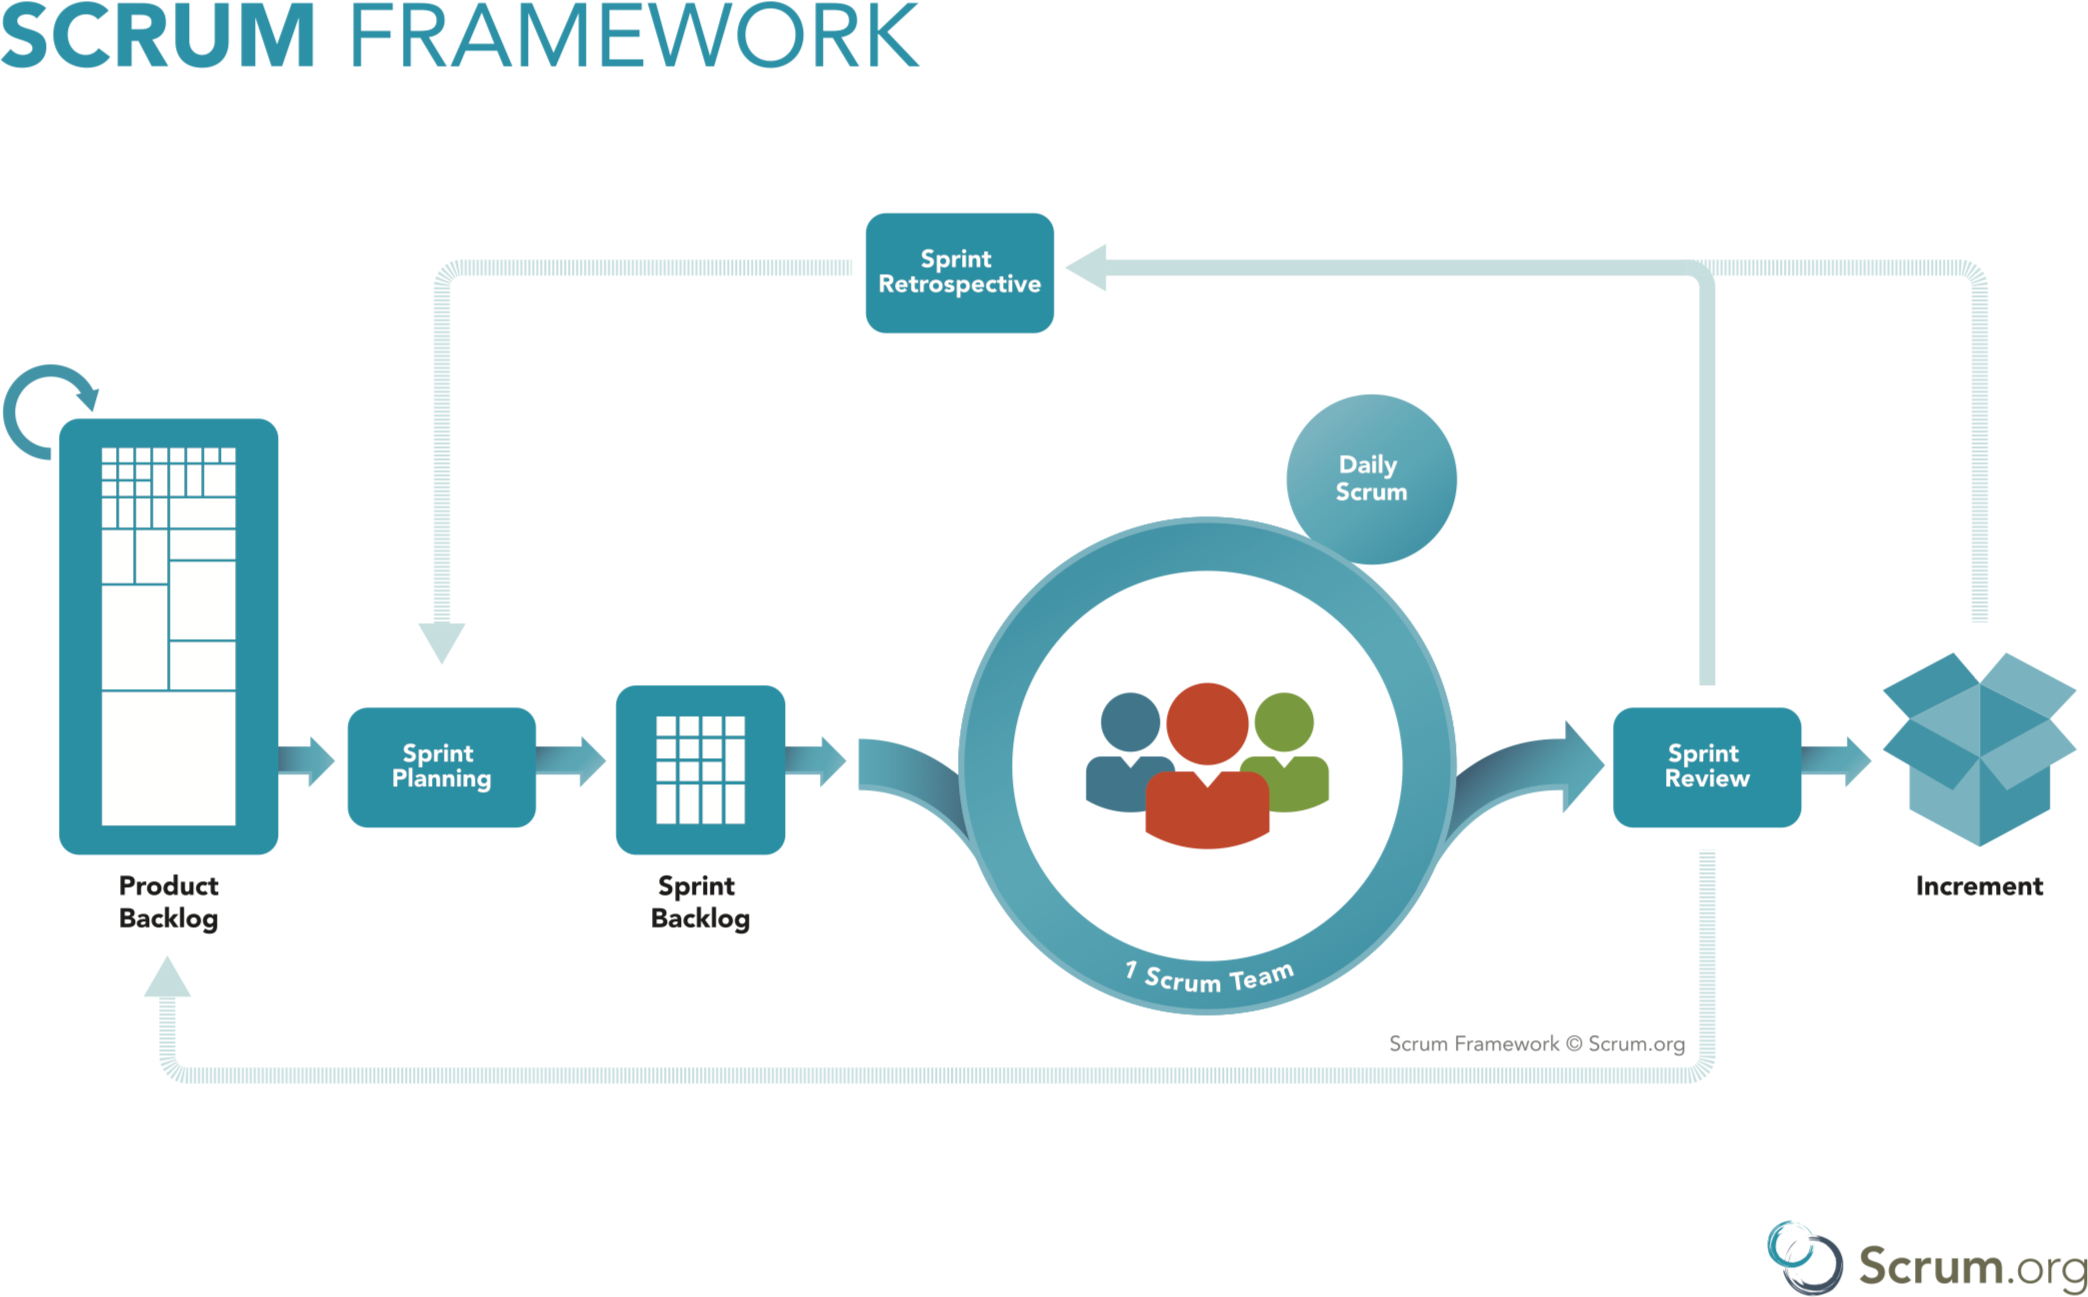
\includegraphics[width=0.9\textwidth]{img/scrum-framework.png}
    \caption[Scrum Framework]{Scrum Framework~\footcite{scrum_framework}}\label{fig:scrum_framework}
  \end{figure}
\end{savenotes}

Das Scrum Framework (Abbildung~\ref{fig:scrum_framework}) besteht aus drei Rollen, fünf Ereignissen und drei Artefakten.

\begin{itemize}
  \item \textbf{Rollen}
  \begin{itemize}
    \item \textbf{Development Team}: Selbstorganisiertes Team, das am Produkt arbeitet.
    \item \textbf{Scrum Mater}: Verantwortlich dafür, sicherzustellen, dass Scrum verstanden und gelebt wird.
    \item \textbf{Product Owner}: Verantwortlich den Wert des Produktes und die Arbeit des Development Teams zu maximieren.
  \end{itemize}
  \item \textbf{Ereignisse}
  \begin{itemize}
    \item \textbf{Sprint}: Ist das Herz von Scrum: eine Timebox von 2 bis 4 Wochen, in dem ein fertiges, verwendbares und potentiell releasebares Produkt-Inkrement entwickelt wird.
    \item \textbf{Sprint Planning}: Planung eines Sprints. Hier commited sich das Scrum Team, eine gewisse Anzahl an Aufgaben im kommenden Sprint abzuarbeiten.
    \item \textbf{Daily Scrum}: Tägliches, zeitlich begrenztes Meeting, bei dem von jedem Teammitglied folgende drei Fragen beantwortet werden:
    \begin{enumerate}
      \item Was habe ich gemacht?
      \item Was werde ich machen?
      \item Was behindert mich bei meiner Arbeit?
    \end{enumerate}
    \item \textbf{Sprint Review}: Abschluss eines Sprints. Hier präsentiert das Team dem Product Owner die Ergebnisse des letzten Sprints.
    \item \textbf{Sprint Retrospective}: Das Team reflektiert den Sprint-Ablauf und ergreift Maßnahmen, um den Prozess weiter zu verbessern.
  \end{itemize}
  \item \textbf{Artefakte}
  \begin{itemize}
    \item \textbf{Product Backlog}: Ist eine Sammlung von möglichen Aufgaben für das Team am Produkt. Sollte einen Ausblick auf die zukünftige Entwicklung des Produktes geben. Oben im Product Backlog befinden sich die bereits fein geplanten Aufgaben, weiter unten die groben.
    \item \textbf{Sprint Backlog}: Entspricht den Aufgaben, die vom Team in den Sprint genommen und dem Product Owner zugesagt wurden.
    \item \textbf{Increment}: Entsteht am Ende eines jeden Sprints und ist eine lauffähige Version des Produkts, die releasefähig ist.
  \end{itemize}
\end{itemize}

\subsection[Scrum in mehreren Teams]{Scrum in mehreren Teams~\footcite[vgl.][S.172ff]{scrum_kurz_gut_2013}}

Scrum beschreibt eine agile Vorgehensweise für ein Team (ein Team entwickelt ein Produkt).
In der Realität existieren aber oft mehrere Teams und/oder mehrere Produkte. 
Dahingehend muss die Organisation der unterschiedlichen Scrum Teams individuell angepasst werden.
Für die Trennung der Teams gibt es unterschiedliche Ansätze:
\begin{description}
  \item[Trennung nach Organisationseinheiten] \hfill \\ Die Teams werden entlang der Abteilungsstruktur einer Organisation getrennt. Aus Scrum-Sicht macht das nicht immer Sinn, da bei der Umsetzung eines Features Abhängigkeiten zu anderen Teams bestehen (keine cross-funktionalen Teams).
  \item[Trennung nach Komponenten (Komponenten-Teams)] \hfill \\ Die technischen Komponenten werden den Teams zugeteilt, was ebenfalls zu Abhängigkeiten zu anderen Teams führt und eine gute Abstimmung zwischen den Teams voraussetzt.
  \item[Trennung nach fachlichen Themen (Feature-Teams)] \hfill \\ Jedes Team entwickelt, unabhängig von den anderen Teams, eine fachliche Komponente. Diese Variante erfüllt die Forderung des Scrum Frameworks nach cross-funktionalen Teams, weshalb bei dieser Form die Abstimmung zwischen den Teams am geringsten ist.
\end{description}

\begin{savenotes}
  \begin{figure}[H]
    \centering
    \subfigure[Feature-Teams]{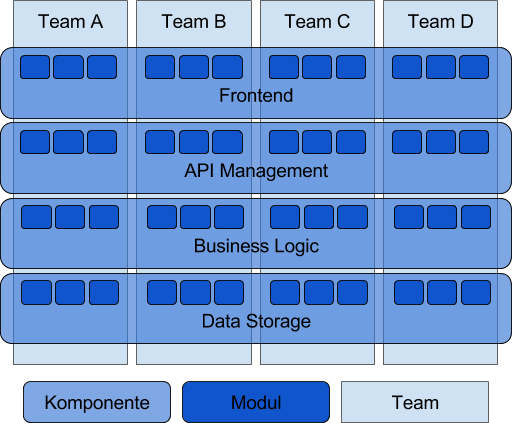
\includegraphics[width=0.40\textwidth]{img/feature-teams.png}} 
    \subfigure[Komponenten-Teams]{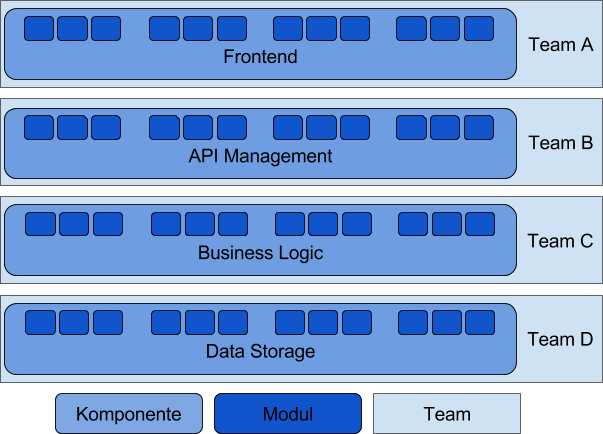
\includegraphics[width=0.48\textwidth]{img/component-teams.png}} 
  \caption{Scrum Teams}\label{fig:Scrum Teams}
  \end{figure}
\end{savenotes}

In allen Varianten existieren aber pro Team unterschiedliche Software-Module und (agile) Prozesse, die unabhängig voneinander die Team-Qualität als Gesamtes bestimmen.
\\
\\
Um Scrum auf mehrere Teams skalieren zu können, existieren bereits unterschiedlichste Frameworks.
Drei davon sind \ac{SoS}, \ac{LeSS} und Scrum at Scale, die im Folgenden kurz vorgestellt werden.

\newpage
\subsubsection[\ac{SoS}]{\ac{SoS}~\footcite[vgl.][]{sos}}

\ac{SoS} ist eine Technik, um Scrum auf große Gruppen zu skalieren. 
Dabei werden die Gruppen in agile Teams von fünf bis zehn Personen geteilt.
Nach jedem Daily Scrum wird pro Team ein Botschafter bestimmt, um an einem täglichen Meeting mit anderen Botschaftern teilzunehmen, das sogenannte Scrum of Scrums.
Je nach Kontext sind die Botschafter technische Teilnehmer, Scrum Master oder sogar Team Manager.
Das \ac{SoS} hat sein eigenes Backlog, bei dem es Fertigstellungen, nächste Schritte und Hindernisse im Auge behält.

\begin{savenotes}
  \begin{figure}[H] 
    \centering
       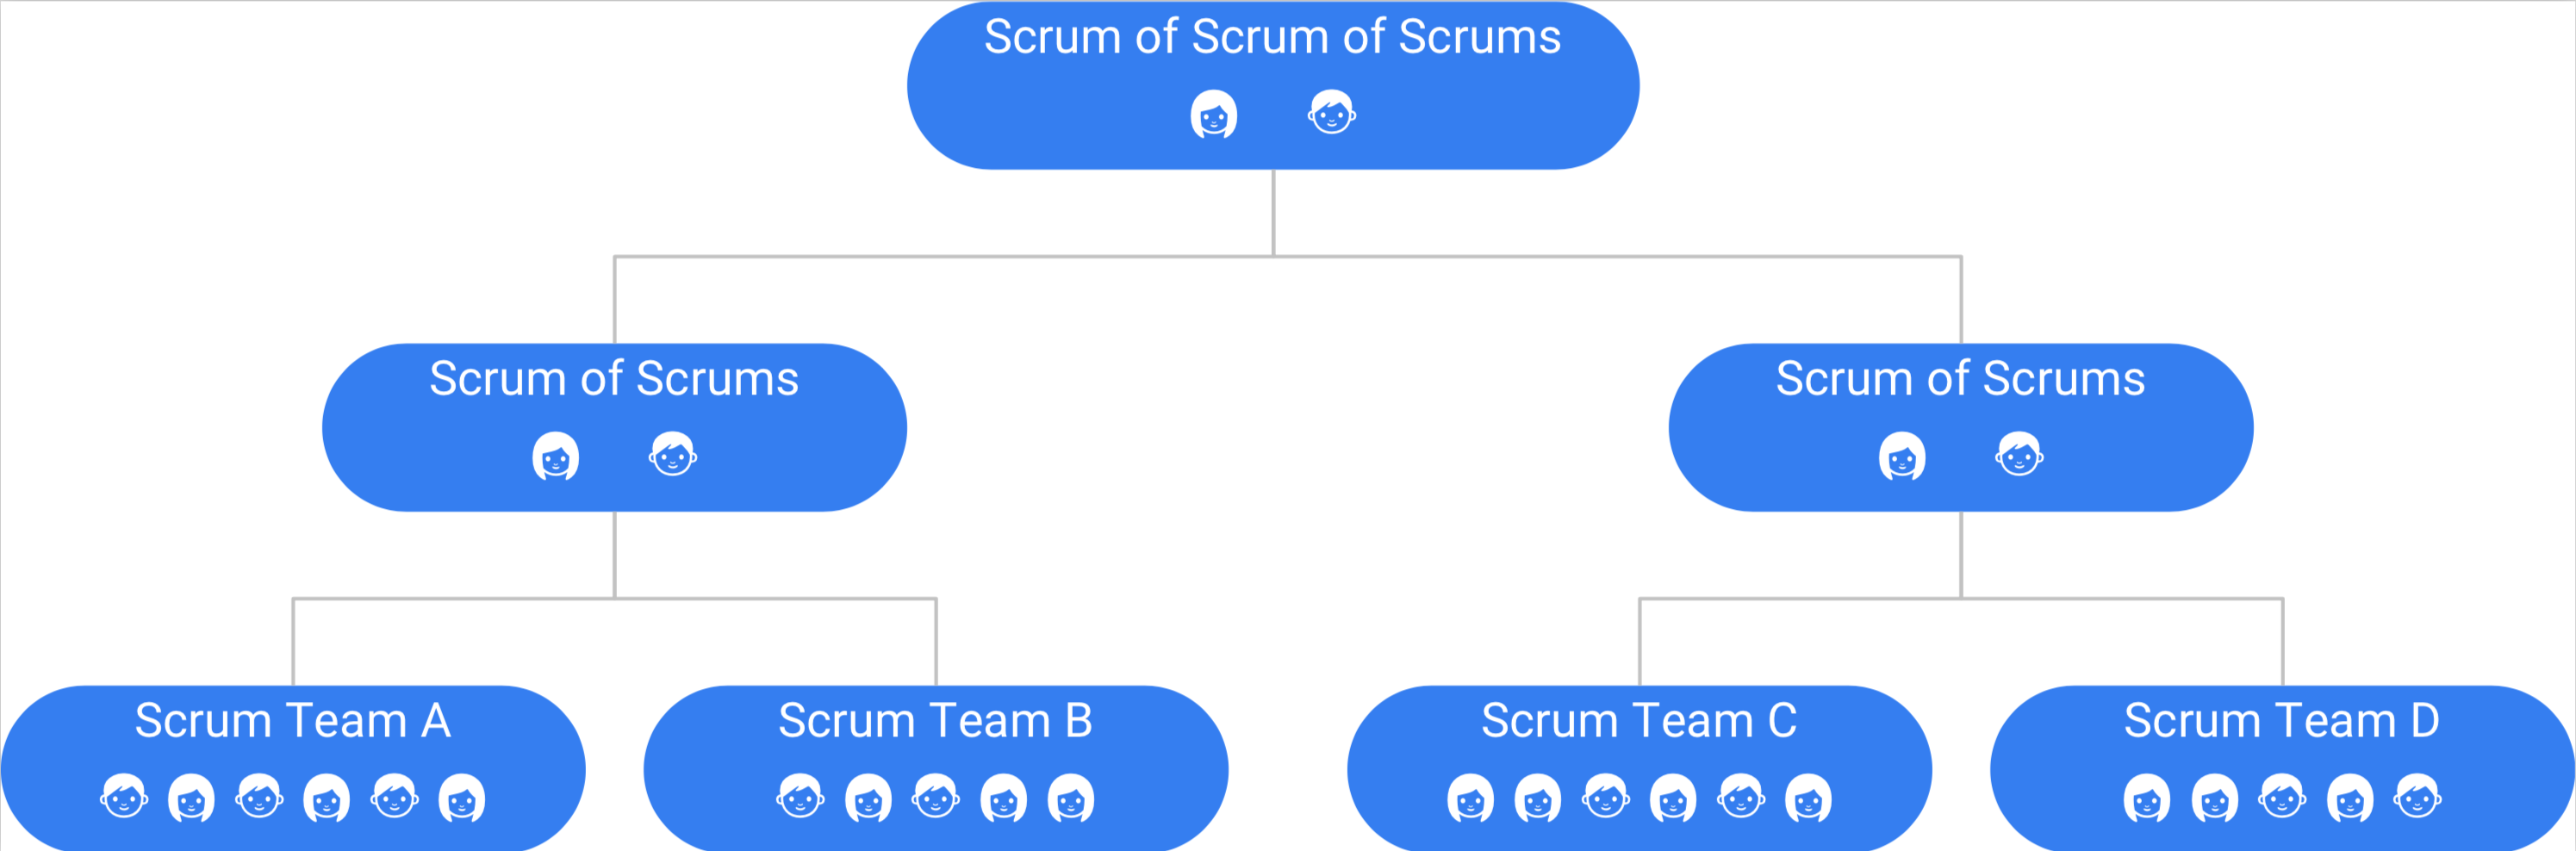
\includegraphics[width=1.0\textwidth]{img/sos.png}
    \caption{\ac{SoS} auf 3 Ebenen}\label{fig:sos}
  \end{figure}
\end{savenotes}

\ac{SoS} ist beliebig skalierbar, das ermöglicht auch mehrere Scrum of Scrums Ebenen, wie Abbildung~\ref{fig:sos} zeigt.

\subsubsection[\ac{LeSS}]{\ac{LeSS}~\footcite[vgl.][]{less}}

\ac{LeSS} adaptiert die Grundsätze von Scrum in einen größeren Rahmen.
Daher muss auch zuerst Scrum für ein Team verstanden werden, bevor mit \ac{LeSS} begonnen werden kann.
Es unterscheidet dabei zwei Varianten:
\begin{description}
  \item[LeSS] für bis zu 8 Teams mit jeweils acht Mitgliedern
  \item[LeSS Huge] bis zu mehrere tausend Personen an einem Produkt
\end{description}

\begin{savenotes}
  \begin{figure}[H] 
    \centering
       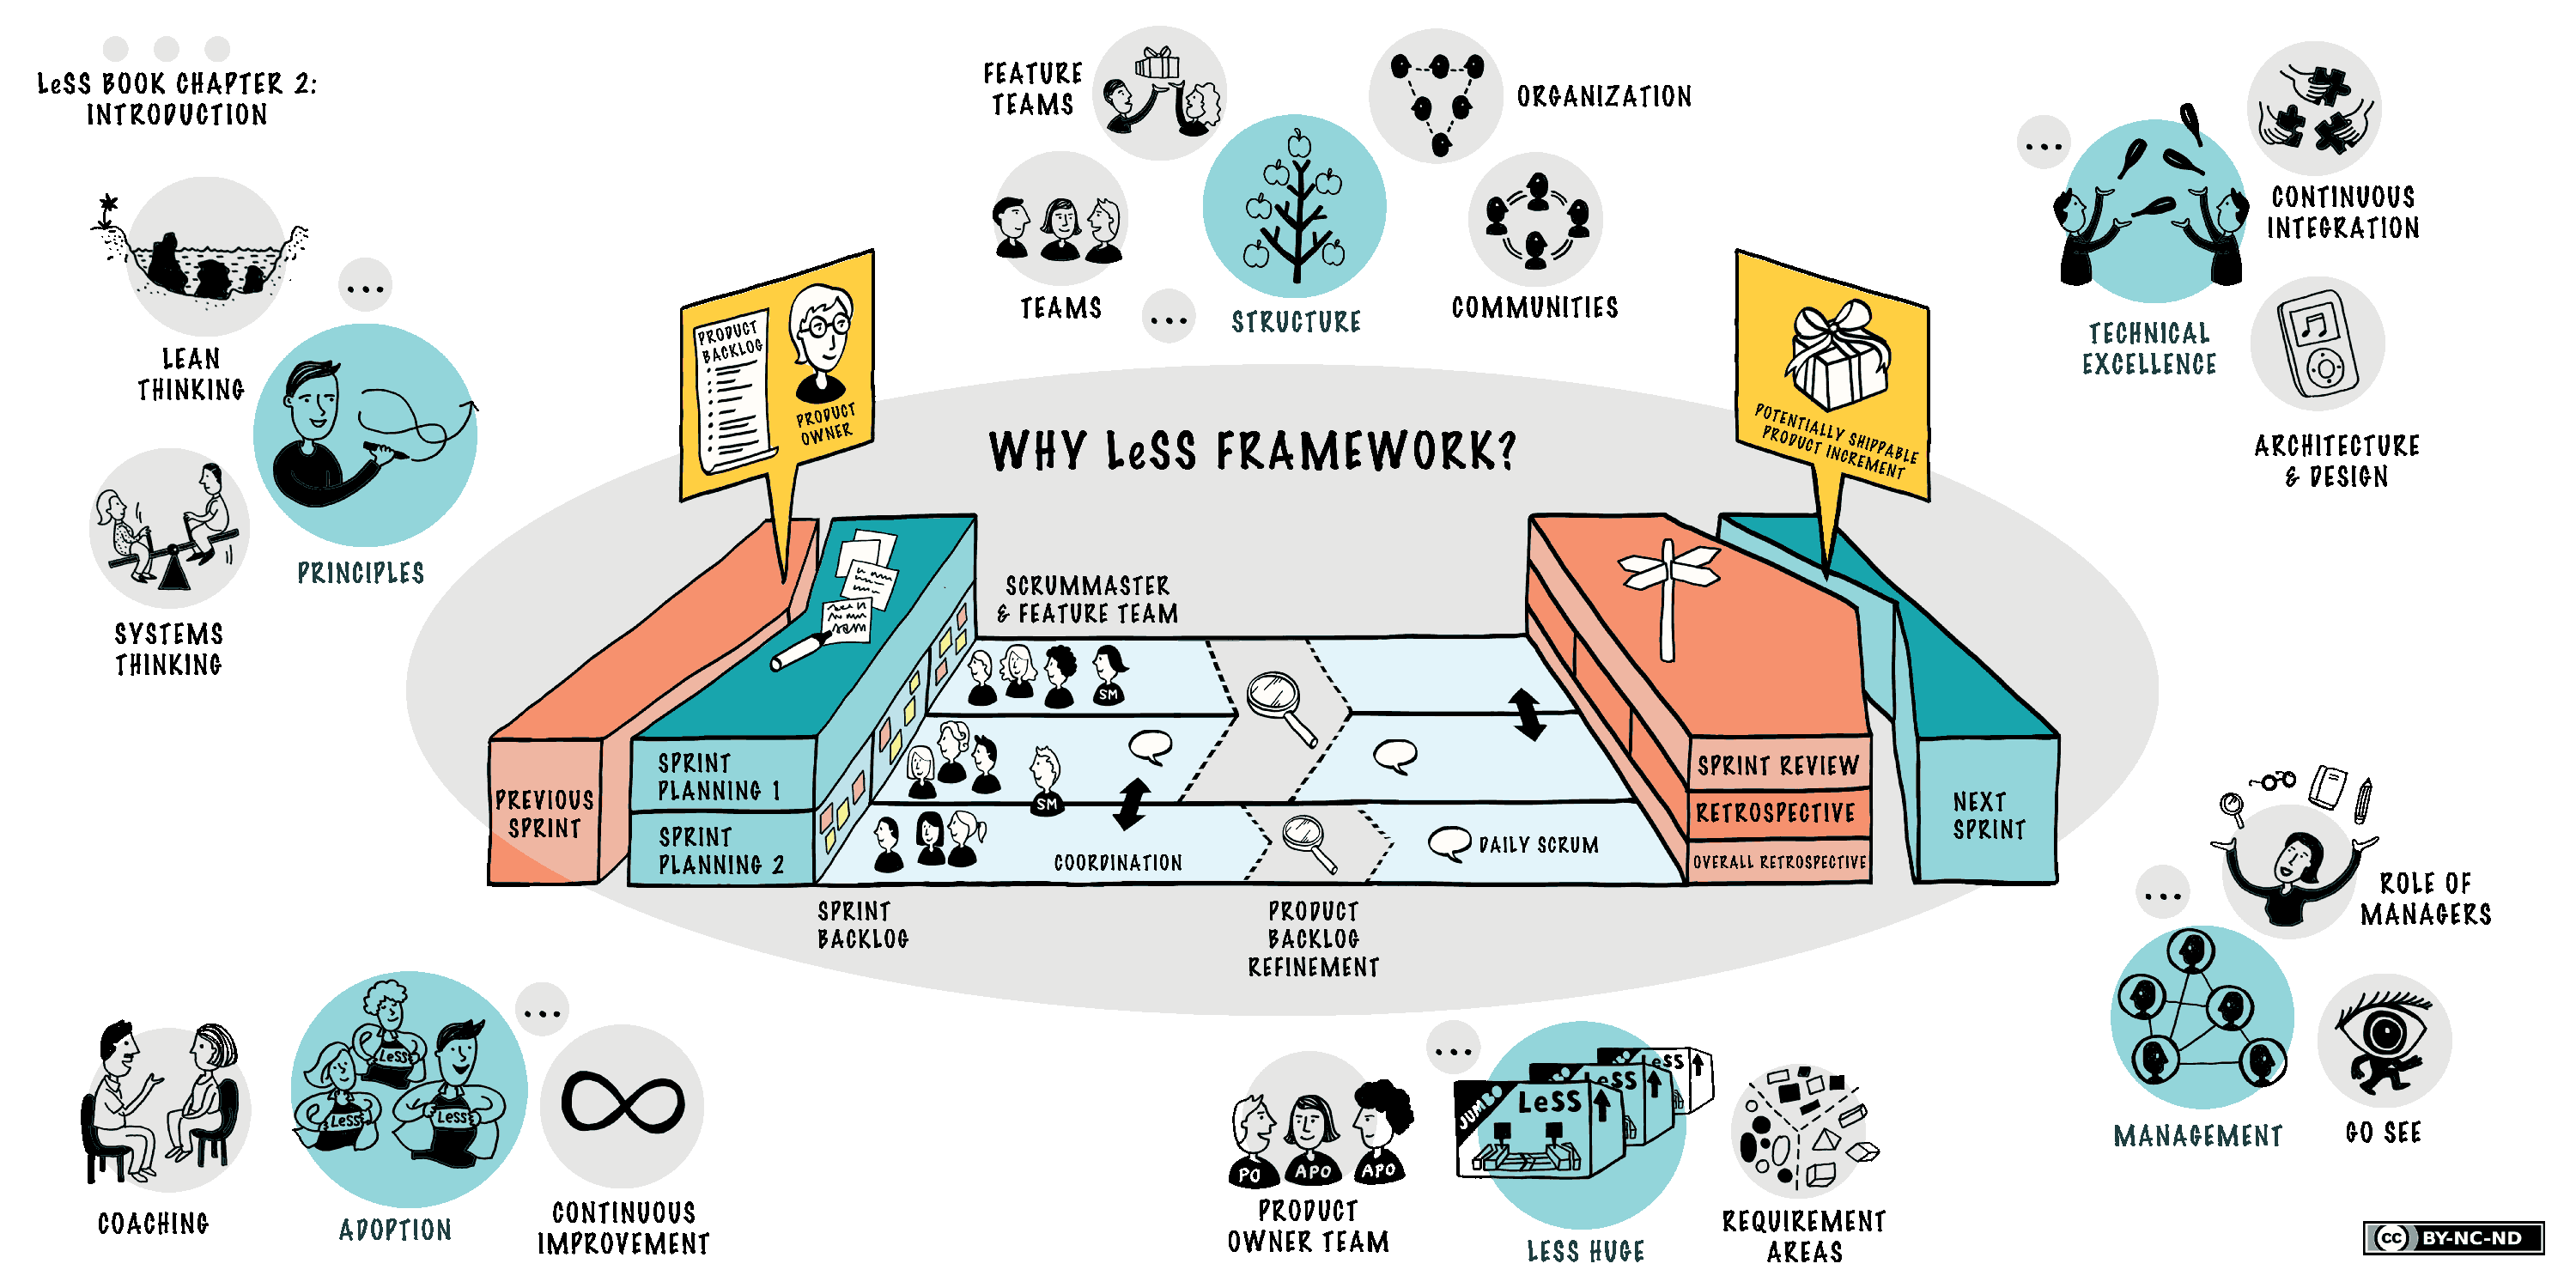
\includegraphics[width=1.0\textwidth]{img/less.png}
    \caption[\ac{LeSS} Framework]{\ac{LeSS} Framework~\footcite{less_framework}}\label{fig:less}
  \end{figure}
\end{savenotes}

Es gibt viele Dinge, die gleich bleiben, wie bei einem Team: Produkt Backlog, \ac{DoD}, nach jedem Sprint ein lauffähiges Inkrement, Product Owner, cross-funktionale Teams und ein Sprint.
Darüber hinaus gibt es aber auch einige Unterschiede:

\begin{description}
  \item[Sprint Planning 1] kann Personen von allen Teams beinhalten, die sich ihre Arbeit selbstständig aufteilen.
  \item[Sprint Planning 2] wird von jedem Team selbst abgehalten, es können aber mehrere Teams in einem Raum sein.
  \item[Daily Scrum] wird auch unabhängig in jedem Team abgehalten, aber eine Person aus Team A kann bei Team B dabei sein, um den Informationsfluss zu erhöhen.
  \item[Overall \ac{PBR}] ist kurz und informativ, um abzuklären, welches Team vermutlich welche Aufgabe übernimmt, für das spätere \ac{PBR}.
  \item[\ac{PBR}] können auch mehrere Teams gemeinsam machen, um voneinander zu lernen und besser koordinieren zu können.
  \item[Sprint Review] kann zusätzlich Personen aus anderen Teams oder andere Steakholder beinhalten.
  \item[Overall Retrospective] ist ein ganz neues Meeting mit Scrum Mastern, Product Ownern und rotierenden Personen der Teams, um den Gesamtprozess zu verbessern.
\end{description}

\subsubsection[Scrum at Scale]{Scrum at Scale~\footcite[vgl.][]{scale}}

Scrum at Scale versucht Scrum skalierbar zu machen, durch ein Minimum an Bürokratie und einer frei skalierbaren Architektur.
Es besteht aus Scrum Teams, die durch \ac{SoS} und MetaScrums koordiniert werden. 
\begin{savenotes}
  \begin{figure}[H] 
    \centering
       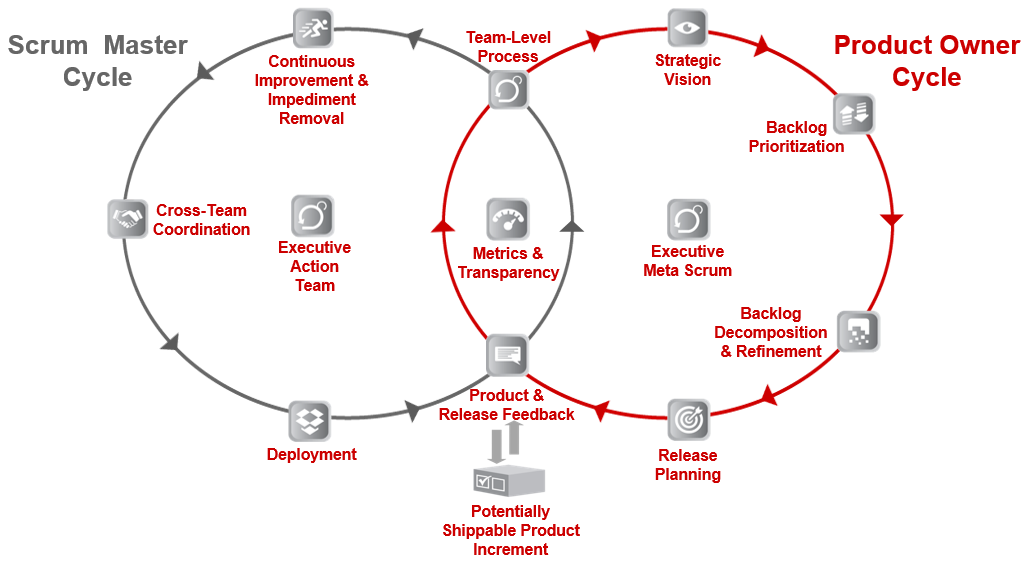
\includegraphics[width=1.0\textwidth]{img/scrumatscale.png}
    \caption[Scrum at Scale Framework - SMPO Zyklus]{Scrum at Scale Framework - SMPO Zyklus~\footcite{scrumatscale_framework}}\label{fig:sas}
  \end{figure}
\end{savenotes}

Das Was und das Wie werden bei Scrum at Scale durch zwei Zyklen getrennt, die sich nur an zwei Punkten schneiden (Abbildung~\ref{fig:sas}).
\begin{description}
  \item[Scrum Master Zyklus] \hfill \\ Wird über \ac{SoS} gesteuert und hat an der Spitze ein \ac{EAT}, welches die einzelnen \ac{SoS} koordiniert.
  \item[Product Owner Zyklus] \hfill \\ Ein Team von Product Ownern, die ein \ac{SoS} Backlog verantworten, nennt man MetaScrum. MetaScrums haben einen Chief Product Owner, der als Scrum Master agiert und verantwortlich für die Koordination der Product Backlogs ist. An der Spitze steht ein \ac{EMS}, der Visionen und strategische Ziele verfolgt.
\end{description}

Metriken und Transparenz im Allgemeinen werden bei Scrum at Scale groß geschrieben, da Scrum nur so optimal funktionieren kann.
Ein Minimum an Metriken, die empfohlen werden, sind: Produktivität, Wertschöpfung, Qualität und Nachhaltigkeit.

\clearpage
\section[Software-Qualität]{Software-Qualität~\footcite[vgl.][Kapitel 1.2]{hoffmann_software_qualitat_2013}}

Eine mögliche Definition von Software-Qualität findet sich in der DIN-ISO-Norm 9126:

\begin{quote}
  ``Software-Qualität ist die Gesamtheit der Merkmale und Merkmalswerte eines Software-Produkts, die sich auf dessen Eignung beziehen, festgelegte Erfordernisse zu erfüllen.''
\end{quote}

Wie aus dieser Definition schon erkennbar ist, gibt es viele unterschiedliche Kriterien, um die Qualität von Software zu bewerten.
Einige wesentliche Merkmale, um die Qualität von Software bewerten zu können, lassen sich in kunden- und herstellerorientierte Merkmale unterteilen:

\begin{description}
  \item[Kundenorientierte Merkmale] \hfill \\ Nach außen hin sichtbare Merkmale, die sich auf den kurzfristigen Erfolg der Software auswirken, da sie die Kaufentscheidung möglicher Kunden beeinflussen.
  \begin{description}
    \item[Funktionalität (Functionality, Capability)] \hfill \\ Beschreibt die Umsetzung der funktionalen Anforderungen. Fehler sind hier häufig Implementierungsfehler (sogenannte Bugs), welche durch Qualitätssicherung bereits in der Entwicklung entdeckt oder vermieden werden können. 
    \item[Laufzeit (Performance)] \hfill \\ Beschreibt die Umsetzung der Laufzeitanforderungen. Besonderes Augenmerk muss in Echtzeitsystemen auf dieses Merkmal gelegt werden.
    \item[Zuverlässigkeit (Reliability)] \hfill \\ Eine hohe Zuverlässigkeit ist in kritischen Bereichen, wie z.B. Medizintechnik oder Luftfahrt, unabdingbar. Erreicht werden kann diese aber nur durch die Optimierung einer Reihe anderer Kriterien.
    \item[Benutzbarkeit (Usability)] \hfill \\ Betrifft alle Eigenschaften eines Systems, die mit der Benutzer-Interaktion in Berührung kommen.
  \end{description}
  \item[Herstellerorientierte Merkmale] \hfill \\ Sind die inneren Merkmale, die sich auf den langfristigen Erfolg der Software auswirken und somit als Investition in die Zukunft gesehen werden sollten.
  \begin{description}
    \item[Wartbarkeit (Maintainability)] \hfill \\ Die Fähigkeit auch nach der Inbetriebnahme noch Änderungen an der Software vorzunehmen. Wird oft vernachlässigt, ist aber essentiell für langlebige Software und ein großer Vorteil gegenüber der Konkurrenz.
    \item[Transparenz (Transparency)] \hfill \\ Beschreibt, wie die nach außen hin sichtbare Funktionalität intern umgesetzt wurde. Gerade bei alternder Software, kann es zu einer Unordnung kommen, welche auch Software-Entropie (Grad der Unordnung) genannt wird.
    \item[Übertragbarkeit] \hfill \\ Wird auch Portierbarkeit genannt und beschreibt die Eigenschaft einer Software, in andere Umgebungen übertragen werden zu können (z.B. 32-Bit zu 64-Bit oder Desktop zu Mobile).
    \item[Testbarkeit (Testability)] \hfill \\ Testen stellt eine große Herausforderung dar, da oft auf interne Zustände zugegriffen werden muss oder die Komplexität die möglichen Eingangskombinationen vervielfacht. Aber gerade durch Tests können Fehler frühzeitig entdeckt und behoben werden.
  \end{description}
\end{description}

Je nach Anwendungsgebiet und den Anforderungen der Software haben die Merkmale unterschiedliche Relevanz und einige können sich auch gegenseitig beeinflussen, wie aus der Korrelationsmatrix in Abbildung~\ref{fig:scrum_framework} ersichtlich.
Dabei sind die positiv korrelierenden Merkmale mit ``+'' und die negativ korrelierenden mit ``-'' gekennzeichnet.

\begin{savenotes}
  \begin{figure}[H] 
    \centering
       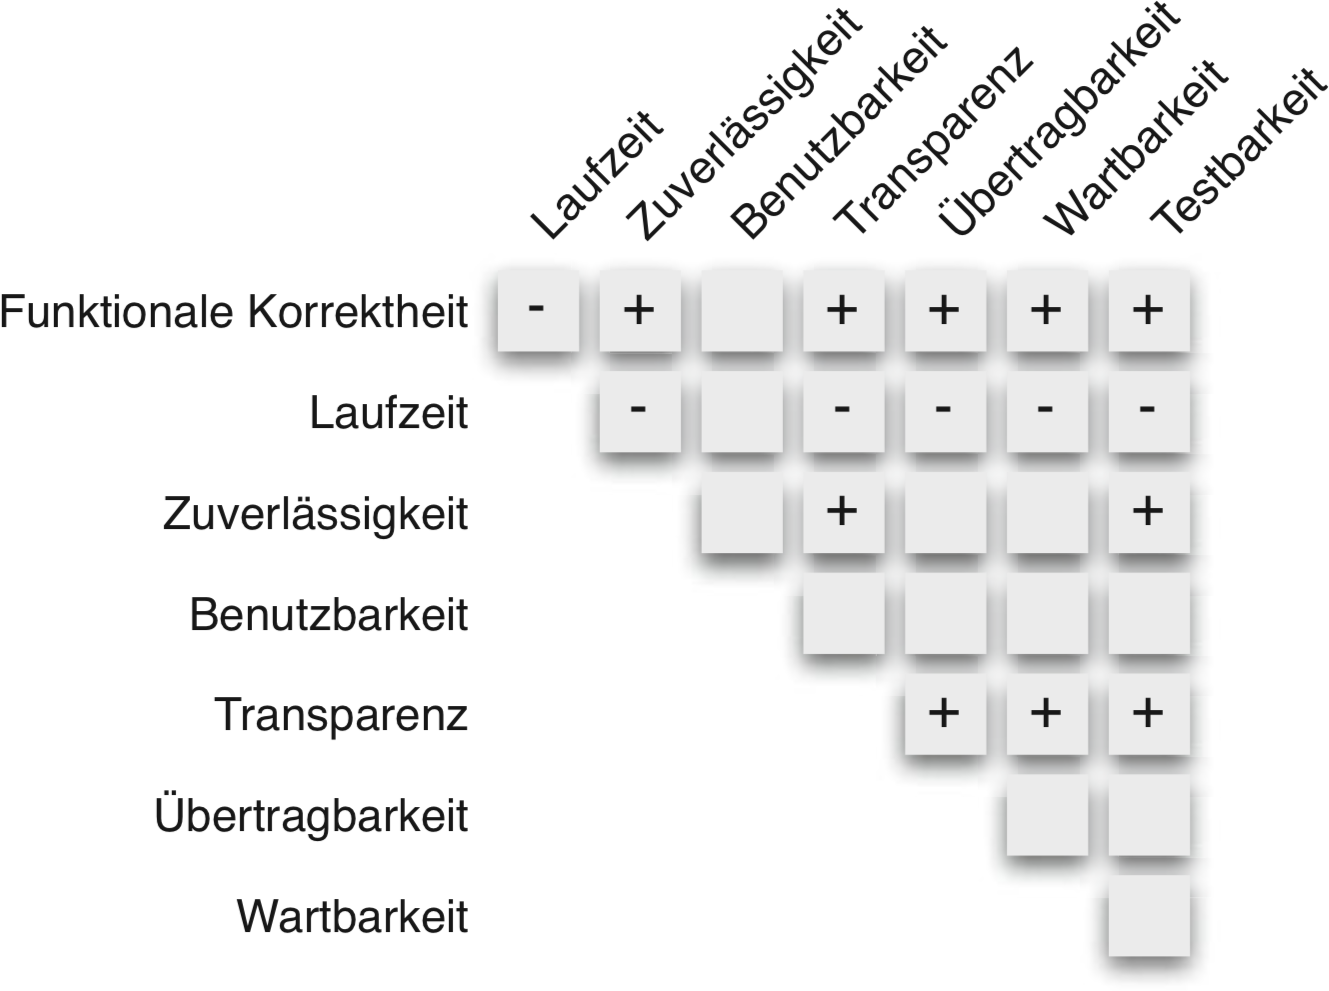
\includegraphics[width=0.6\textwidth]{img/korrelationsmatrix-kriterien.png}
    \caption[Korrelationsmatrix Qualitätskriterien]{Korrelationsmatrix Qualitätskriterien~\footcite[][S. 11, Abb. 1.3]{hoffmann_software_qualitat_2013}}\label{fig:Korrelationsmatrix Qualitätskriterien}
  \end{figure}
\end{savenotes}

\newpage
\section{Metriken}

Eine Softwaremetrik wird vom \ac{IEEE} Standard 1061 von 1998 folgendermaßen definiert:
\begin{quote}
  ``Eine Softwarequalitätsmetrik ist eine Funktion, die eine Software-Einheit in einen Zahlenwert abbildet, welcher als Erfüllungsgrad einer Qualitätseigenschaft der Software-Einheit interpretierbar ist.''\footcite[vgl.][S.3]{ieee-1061}
\end{quote}

Vereinfacht gesagt, ist eine Metrik eine oder mehrere Kennzahlen, die mithilfe einer Funktion ein Qualitätsmerkmal in einen Zahlenwert abbilden.
Eine Kennzahl kann daher auch schon direkt eine Metrik sein, wenn sie in der Lage ist, ein gewünschtes Qualitätsmerkmal abzubilden.

\begin{savenotes}
  \begin{figure}[H] 
    \centering
       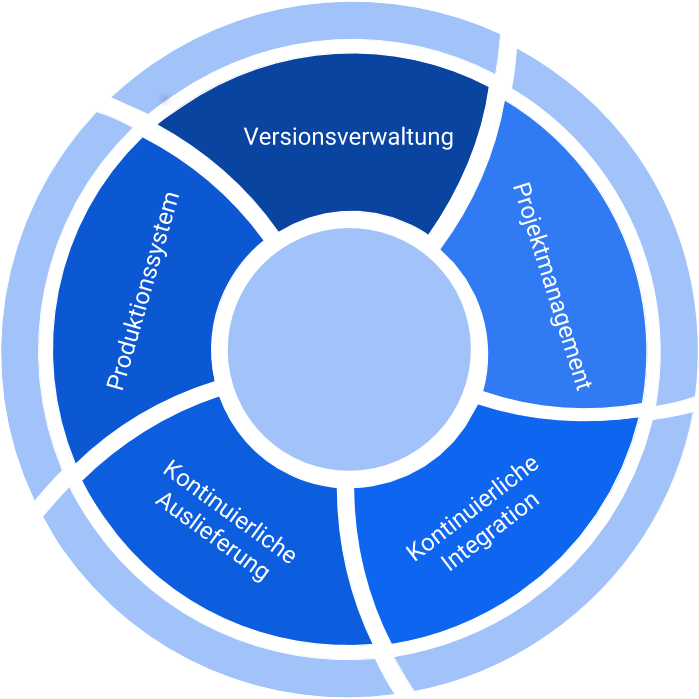
\includegraphics[width=0.6\textwidth]{img/software-development-lifecycle.png}
    \caption[Systeme im Softwareentwicklungsprozess]{Systeme im Softwareentwicklungsprozess~\label{fig:sdlc}}
  \end{figure}
\end{savenotes}

Im Entwicklungsprozess werden in den unterschiedlichen Systemen und Prozessschritten Daten erzeugt, die als Kennzahlen oder direkt als Metriken genutzt werden können.
Abbildung~\ref{fig:sdlc} zeigt die einzelnen Schritte und Systeme im Entwicklungsprozess.

\newpage
\subsection[Versionsverwaltung]{Versionsverwaltung~\footcite[vgl.][S.62ff]{davis_agile_2015}}

Das \ac{VCS} befindet sich nah an der Arbeit der Entwickler, da hier der Quellcode des Produkts verwaltet wird.
Daher können hier Daten darüber gesammelt werden, wie viel gearbeitet und auch wie viel zusammengearbeitet wird.
Um bestmögliche Daten zu bekommen, sollten verteilte Versionskontrollsysteme wie Git verwendet und mit Pull Requests gearbeitet werden.

\begin{description}
  \item[\ac{CLOC}] \hfill \\ Anzahl der geänderten Code Zeilen.
  \item[\ac{CLOC} pro Entwickler] \hfill \\ Anzahl der geänderten Zeilen im Quellcode pro Entwickler.
  \item[Commits] \hfill \\ Gesamtzahl an Commits in einem bestimmten Zeitraum.
  \begin{description}
    \item[Commits pro Entwickler] \hfill \\ Gesamtzahl an Commits in einem bestimmten Zeitraum pro Entwickler.
    \item[Kommentare pro Commit] \hfill \\ Anzahl der Kommentare pro Commit.
    \item[\ac{CLOC} pro Commit] \hfill \\ Anzahl der geänderten Zeilen im Quellcode pro Commit.
  \end{description}
  \item[Pull Requests] \hfill \\ Gesamtzahl an Pull Requests in einembestimmten Zeitraum.
  \begin{description}
    \item[Gemergte Pull Requests] \hfill \\ Anzahl erfolgreicher Pull Requests ineinem bestimmten Zeitraum.
    \item[Abgelehnte Pull Requests] \hfill \\ Anzahl abgelehnter Pull Requests in einem bestimmten Zeitraum.
    \item[Kommentare pro Pull Request] \hfill \\ Anzahl der Kommentare pro Pull Request.
  \end{description}
\end{description}

\newpage
\subsection[Projektmanagement]{Projektmanagement~\footcite[vgl.][S.37ff]{davis_agile_2015}}

In einem \ac{PTS} werden Aufgaben definiert und zugewiesen, Bugs verwaltet und Arbeitszeit mit Aufgaben verknüpft.
Hier können Daten über das Projektverständnis des Teams, die Geschwindigkeit und vor allem die Konsistenz der Arbeit gesammelt werden.
Um bestmögliche Daten erhalten zu können, gibt es folgende Empfehlungen:
\begin{itemize}[noitemsep]
  \item \ac{PTS} wird von allen genutzt
  \item Aufgaben mit möglichst vielen Tags versehen
  \begin{itemize}
    \item Aufgaben kategorisieren (nach ``gut'', ``ok'' und ``schlecht'')
  \end{itemize}
  \item Aufgaben schätzen
  \item gemeinsam eine \ac{DoD} festlegen
\end{itemize}
Jede Arbeit, die am \ac{PTS} vorbei geht, fällt später bei der Auswertung der Daten durch das Raster.
Durch das Taggen der Aufgaben können später Korrelationen ausgewertet werden, vor allem auch durch das Taggen, wie gut die Aufgabe abgelaufen ist.
Nur wenn die Aufgabe geschätzt ist, kann festgestellt werden, ob richtig geschätzt wurde oder wie viele Ausreißer es gibt. Dazu muss auch die Arbeitszeit auf der Aufgabe gespeichert werden.
Die \ac{DoD} hilft allgemein den Prozess zu verbessern und Rückläufe im Arbeitsablauf zu minimieren.

Dadurch ergeben sich folgende Kennzahlen aus einem \ac{PTS}:
\begin{description}
  \item[Burn Down] \hfill \\ Die Anzahl erledigte Arbeit über die Zeit. Liefert einen Richtwert, wo man sich gerade im Sprint befindet, verglichen zum Commitment.
  \item[Velocity] \hfill \\ Eine relative Messung der Konsistenz erledigter Arbeit über die Sprints.
  \item[Cummulative Flow] \hfill \\ Zeigt wie viel Aufgaben nach Status dem Team zugewiesen sind über die Zeit.
  \item[Lead Time] \hfill \\ Zeit zwischen Start und Abschluss einer Aufgabe, vor allem interessant bei Kanban.
  \item[Bug Counts] \hfill \\ Die Anzahl an Bugs über die Zeit.
  \begin{description}
    \item[Bug-Erzeugungsrate] \hfill \\ Anzahl Bugs nach Erstellungsdatum.
    \item[Bug-Fertigstellungsrate] \hfill \\ Anzahl Bugs nach Erledigungsdatum.
  \end{description}
  \item[Aufgaben-Volumen] \hfill \\ Die Anzahl der Aufgaben. Kann der Schätzung gegenübergestellt werden, um die Größe der Aufgaben oder ungeplante Arbeit aufzuzeigen.
  \item[Aufgaben-Rückfälligkeit] \hfill \\ Zeigt auf, wie oft Aufgaben im Arbeitsablauf rückwärts gehen.
\end{description}

\subsection[Kontinuierliche Integration und Auslieferung]{Kontinuierliche Integration und Auslieferung~\footcite[vgl.][S.84ff]{davis_agile_2015}}

\ac{CI}- und \ac{CD}-Systeme stellen sicher, dass die erstellte Software zu jedem Zeitpunkt auslieferbar ist, in dem sie zu definierten Zeitpunkten automatisch neu gebaut und ausgeliefert wird.
In einer solchen Build-Pipeline können sehr viel nützliche Daten erzeugt werden, vor allem mit Tools für statische Analysen (wie zum Beispiel SonarQube~\footcite[][]{sonarqube}).
Diese Systeme sind aber auch jene Elemente im Softwareentwicklungsprozess, die von Team zu Team am meisten variieren können.
Daher hängen die erzeugten Daten auch stark vom jeweiligen Setup ab.
Grundsätzlich können aber folgende Kennzahlen aus diesen Systemen ermittelt werden:

\begin{description}
  \item[Build-Dauer] \hfill \\ Geschätzte und tatsächliche Dauer der Builds.
  \item[Build-Status] \hfill \\ Es können die Anzahl der erfolgreichen und fehlerhaften Builds gegenüber gestellt werden.
  \item[Build-Frequenz] \hfill \\ Wie oft wird ein Build ausgelöst.
  \item[Test Reports] \hfill \\ Anzahl erfolgreicher und fehlerhafter Tests, Gesamtdauer der Tests.
  \item[Code Coverage] \hfill \\ Wie viel Prozent des Quellcodes ist mit Tests abgedeckt.
  \item[Stresstests oder Benchmarking] \hfill \\ Wird oft im Build Prozess mit getestet mit Tools wie JMeter~\footcite[][]{jmeter} oder Gatling~\footcite[][]{gatling}.
\end{description}

\newpage
\subsection[Produktionssystem]{Produktionssystem~\footcite[vgl.][S.107ff]{davis_agile_2015}}

Daten aus den Produktionssystemen können gesammelte \ac{APM}- oder auch \ac{BI}-Kennzahlen sein.
Diese Kennzahlen ermöglichen Aussagen, ob die Kunden zufrieden sind und wie das System arbeitet.
Die \ac{BI}-Kennzahlen sollten möglichst nahe am Entwicklungsteam gehalten werden, damit es verstehen kann, wie die Kunden die Applikation nutzen.
Dazu können Frameworks wie StatsD~\footcite[][]{statsd} und Atlas~\footcite[][]{atlas} verwendet werden.
Im Produktionssystem können folgende Kennzahlen ermittelt werden:

\begin{description}
  \item[CPU Nutzung] \hfill \\ Auslastung der Prozessoren über die Zeit.
  \item[Heap Size] \hfill \\ Auslastung des Heap über die Zeit.
  \item[Fehlerraten] \hfill \\ Anzahl Fehler über die Zeit (kann aus dem Logging kommen).
  \item[Antwortzeiten] \hfill \\ Dauer der Verarbeitung bestimmter Anfragen.
  \item[Benutzeranzahl] \hfill \\ Anzahl gleichzeitiger Benutzer in der Applikation über die Zeit.
  \item[Aufenthaltsdauer] \hfill \\ Verweildauer der Benutzer auf bestimmten Seiten.
  \item[Conversion Rate] \hfill \\ Anzahl Benutzer die zu Kunden wurden.
  \item[Semantisches Logging] \hfill \\ Ermöglicht es, beim Logging strukturierte Daten auszugeben, zum Beispiel: was suchen Benutzer auf bestimmten Seiten.
  \item[Verfügbarkeit] \hfill \\ Verfügbarkeit der Applikation über die Zeit.
\end{description}

\subsection{Übersicht Kennzahlen im Entwicklungsprozess}

Die Metriken finden sich nochmal als Tabelle dargestellt und mit den dazugehötigen Fragen, die sie jeweils beantworten, im Anhang~\ref{appendix:metrics}.

\subsection[Veröffentlichung von Metriken]{Veröffentlichung von Metriken~\footcite[vgl.][S.177ff]{davis_agile_2015}}

Metriken können auf verschiedene Art und Weise veröffentlicht werden. Zwei mögliche Beispiele sind Dashboards oder Emails.
Grundsätzlich sollte beachtet werden, dass man sich bei der Veröffentlichung von Metriken innerhalb der Grenzen und Gewohnheiten des Unternehmens bewegen sollte.
Außerdem sollte auf folgende Punkte geachtet werden:

\begin{description}
  \item[Dashboards] \hfill
  \begin{itemize}[noitemsep]
    \item den Zugriff innerhalb der Firma nicht einschränken
    \begin{itemize}[noitemsep]
      \item aber als intern ansehen
    \end{itemize}
    \item muss nach den Bedürfnissen der Teams anpassbar sein
    \item Metriken werden als Werkzeug gesehen, nicht als Waffe (gegen andere Teams oder Personen)
    \item Page Tracking verwenden, um das Nutzungsverhalten zu verstehen
  \end{itemize}
  \item[Emails] \hfill
  \begin{itemize}[noitemsep]
    \item aus dem Dashboard optional machen (sonst landen sie schnell automatisch im Spam-Ordner)
    \item minimal erforderliche Daten, den Rest verlinken zum Dashboard
    \item den Richtigen Rhytmus finden (zwischen oft genug informieren und nerven)
  \end{itemize}
\end{description}

Arbeitet ein Unternehmen beispielsweise viel mit Reports via Email, dann kann ein reines Dashboard weniger Anerkennung finden. Hier könnte beispielsweise eine Übersicht per Mail versendet und mit Links zum Dashboard versehen werden.

\subsection[Eigene Metriken erstellen]{Eigene Metriken erstellen~\footcite[vgl.][S.127ff]{davis_agile_2015}}

Um eigene Metriken erstellen zu können sind 2 Dinge notwendig:
\begin{itemize}
  \item Daten
  \item eine Funktion, um die Metrik zu berechnen
\end{itemize}

Dabei sollte darauf geachtet werden,
\begin{itemize}
  \item dass man auf die Metrik reagieren kann (Dinge, die einen stören und die man nicht ändern kann, frustrieren oder demotivieren)
  \item dass sich die Metrik nach den Team-Grundsätzen und Kerngeschäften ausrichtet
  \item dass die Metrik für sich alleine stehen kann
\end{itemize}

\subsection[Agile Prinzipien messen]{Agile Prinzipien messen~\footcite[vgl.][S.201ff]{davis_agile_2015}}

Um die agilen Prinzipien messen zu können, muss zuerst herausgefunden werden, was die Kernaussagen dieser Prinzipien sind.
Dies kann zum Beispiel grafisch, durch die Erstellung einer Wortwolke, wie in Abbildung~\ref{fig:wordcloud_principles} ersichtlich, erreicht werden.

\begin{savenotes}
  \begin{figure}[H] 
    \centering
    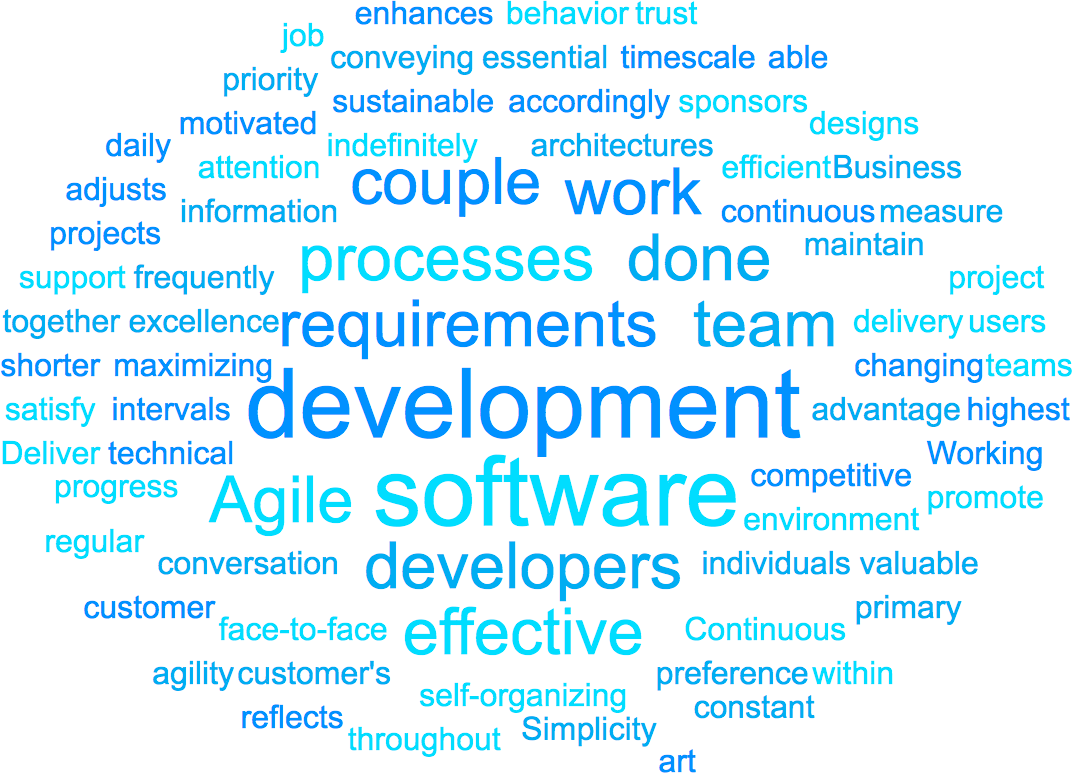
\includegraphics[width=0.9\textwidth]{img/principles-wordcloud.png}
    \caption{Agile Prinzipien als Wortwolke}\label{fig:wordcloud_principles}
  \end{figure}
\end{savenotes}

Aus dieser Wortwolke heben sich neben den Begriffen ``development'' und ``software'' vor allem auch die Begriffe ``team'', ``processes'', ``effective'' und ``requirements'' hervor.
Mithilfe dieser Begriffe lassen sich folgende vier Punkte ableiten:

\begin{itemize}[noitemsep]
  \item Effektive Software
  \item Effektiver Prozess
  \item Effektives Team 
  \item Effektive Anforderungen 
\end{itemize}

Für jeden dieser vier Punkte sind Metriken aus den unterschiedlichsten Systemen anwendbar~\footcite[vgl.][S.219ff]{davis_agile_2015}:

\begin{description}
  \item[Effektive Software] \hfill
  \begin{itemize}[noitemsep]
    \item erfolgreiche / fehlerhafte Builds
    \item Business-Metriken
    \item Status der Applikation
    \begin{itemize}[noitemsep]
      \item Fehlerraten
      \item CPU/Speicher Auslastung
      \item Antwort- / Transaktionszeiten
      \item Heapgröße / Garbage Collection / Anzahl Threads
    \end{itemize}
  \end{itemize}
  \item[Effektiver Prozess] \hfill
  \begin{itemize}[noitemsep]
    \item Velocity
    \item \ac{PTS} und \ac{VCS} Kommentare
    \item erfolgeiche Releases
  \end{itemize}
  \item[Effektives Team] \hfill
  \begin{itemize}[noitemsep]
    \item Lead Time
    \item \ac{MTTR}
    \item Deploy-Frequenz
    \item fehlerhafte Builds
  \end{itemize}
  \item[Effektive Anforderungen] \hfill
  \begin{itemize}[noitemsep]
    \item Rückläufigkeit
    \item Lead Time
    \item \ac{MTTR}
    \item Velocity
  \end{itemize}
\end{description}

\newpage
\subsection{Qualitätsmodelle}

Qualitätsmodelle sind das Fundament für Software-Produkt-Qualitätskontrolle und werden genutzt, um Qualität zu beschreiben, zu schätzen und/oder vorherzusagen.
Es wurden in den letzten Jahrzehnten unzählige Modelle vorgestellt, diese lassen sich in drei Kategorien einteilen: hierarchische, Meta-Modell basierte und implizite Modelle.

\begin{description}
  \item[Hierarchische Qualitätsmodelle] \hfill \\ Entstanden bereits in den 1970er Jahren. Qualität wird hierarchisch in Qualitätsfaktoren zerlegt, wie Wartbarkeit oder Zuverlässigkeit. Die Idee dahinter ist, Qualität hierarchisch herunterzubrechen, dass sie messbar wird. Verschiedenste Kritiken heben hervor, dass die Prinzipien zur Dekomposition von Qualitätscharakteristiken oft mehrdeutig sind. Außerdem sind die resultierenden Qualitätscharakteristiken nicht spezifisch genug, um direkt gemessen werden zu können.
  \item[Meta-Modell basierte Qualitätsmodelle] \hfill \\ Entstanden in den 1990er Jahren, als Forscher mehr ausgereiftere Wege aufzeigten, um Qualitätscharakteristiken zu zerlegen. Dadurch entstanden auch ausführlichere Meta-Modelle. Ein Meta-Modell beschreibt, wie gültig Qualitätsmodelle strukturiert sind. Die vielen Meta-Modelle zeigen, dass Qualität mehr Struktur in Qualitätsmodellen, als in abstrakten Qualitätscharakteristiken und Metriken braucht. Es wurde kein generelles Basis-Qualitätsmodell eingeführt, das man herunterladen und anwenden kann.
  \item[Statistische und implizite Qualitätsmodelle] \hfill \\ Für unterschiedlichste Qualitätsfaktoren wurden statistische Modelle vorgestellt, die Eigenschaften erfassen und Qualitätsfaktoren schätzen oder voraussagen. Auch Qualitäts-Analysetools nutzen eine Art Qualitätsmodell und auch Checklisten in der Entwicklung oder in Reviews sind eine Art Qualitätsmodell.
\end{description}

\newpage
\subsection[\ac{GQM}]{\ac{GQM}~\footcite[][]{basili_goal_nodate}}

\ac{GQM} ist ein Qualitätsmodell, um geeignete Metriken für ein Softwareprojekt finden zu können und wurde ursprünglich von der \ac{NASA} entwickelt, um Fehler in bestimmen Projekten zu erkennen.
Der grundlegende Gedanke dahinter ist, dass Metriken ``top\mbox{-}down'' (von oben nach unten) definiert werden müssen.
Dieser Ansatz wird dadurch begründet, dass Metriken sehr viele Charakteristiken abbilden können, aber erst durch Modelle beziehungsweise Ziele richtig genutzt und interpretiert werden können.

Das Ergebnis dieses Modells hat drei Level:
\begin{description}
  \item[GOAL \mbox{-} konzeptuelles Level] \hfill \\ Es werden Ziele für besimmte Objekte definiert. Objekte können Produkte, Prozesse oder Ressourcen sein.
  \item[QUESTION \mbox{-} operatives Level] \hfill \\ Für jedes Ziel werden Fragen formuliert, die zur Beurteilung oder Erreichung beitragen. Sie versuchen den Grund für die Messung zu charakterisieren.
  \item[METRIC \mbox{-} quantitatives Level] \hfill \\ Jeder Frage werden Metriken zugeordnet, die dabei helfen sollen, sie quantitativ zu beantworten.
\end{description}

\begin{savenotes}
  \begin{figure}[H] 
    \centering
    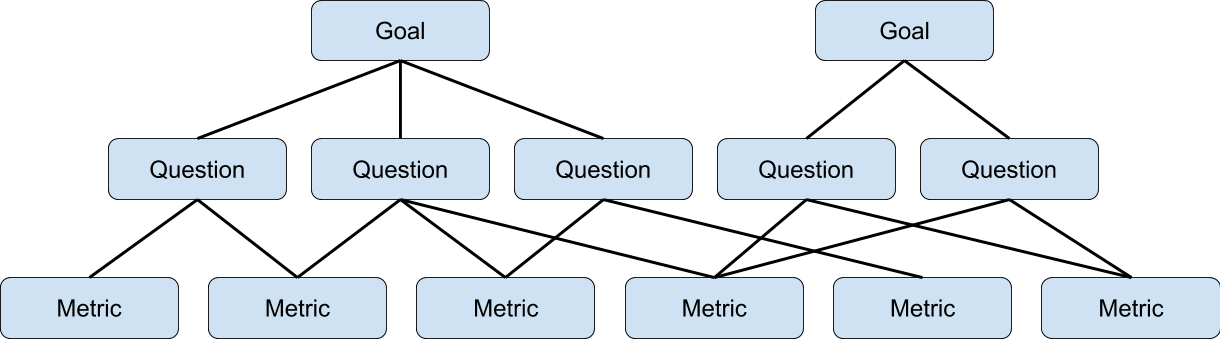
\includegraphics[width=0.9\textwidth]{img/gqm.png}
    \caption{hierarchische Struktur des GQM Modells}\label{fig:gqm}
  \end{figure}
\end{savenotes}

Abbildung~\ref{fig:gqm} zeigt die hierarchische Struktur des GQM-Modells.

\subsubsection[Beispiel]{Beispiel~\footcite[][]{basili_goal_nodate}}

Anhand des Beispiels in Tabelle~\ref{tab:gqm-example} soll veranschaulicht werden, wie so ein GQM-Modell in der Praxis aussehen kann.
Angenommen wird, das Team will seine Zusammenarbeit verbessern. 
Dazu muss das Ziel folgende Punkte spezifizieren: Absicht, Prozess / Produkt / Ressource, Sichtweise und Problem.
Dieses Ziel kann anschließend durch Fragen verfeinert werden.
Aussagen über Zusammenarbeit geben zum Beispiel Pull Requests.
Diese Fragen wiederum können mit Metriken beantwortet werden.
Im Falle der Pull Requests zum Beispiel der Durchschnitt und die Standardabweichung der Kommentare pro Pull Request in jedem Sprint.

\begin{table}[H]
  \centering
  \begin{tabular}{llr}
  GOAL     & \begin{tabular}[c]{@{}l@{}}Absicht\\ Problem\\ Prozess\\ Sichtweise\end{tabular} & \begin{tabular}[c]{@{}l@{}}Verbessern\\ der Zusammenarbeit innerhalb des Teams\\ im Entwicklungsprozess\\ aus Sicht der Entwickler.\end{tabular} \\ \midrule
  QUESTION & \multicolumn{2}{l}{Wie arbeitet das Team mit Pull Requests?} \\
  METRIC   & \multicolumn{2}{l}{\begin{tabular}[c]{@{}l@{}}Anzahl Pull Requests\\ Anzahl Kommentare pro Pull Request *\\ Anzahl Entwickler pro Pull Request *\end{tabular}} \\ \midrule
  QUESTION & \multicolumn{2}{l}{Wie viele Entwickler arbeiten an den einzelnen Modulen?} \\
  METRIC   & \multicolumn{2}{l}{\begin{tabular}[c]{@{}l@{}}Anzahl Commits pro Entwickler pro Modul\\ Anzahl Entwickler pro Pull Request pro Modul *\end{tabular}} \\
  \multicolumn{3}{l}{\begin{tabular}[c]{@{}l@{}} \\ \small{* Durchschnitt und Standardabweichung pro Sprint}\end{tabular}} 
  \end{tabular}
  \caption{Beispiel GQM Modell}\label{tab:gqm-example}
\end{table}

\subsection{Umfrage (Quelle fehlt)}

Quellen zu wissenschaftlichen Umfragen finden, passende einfügen.
Grundsätzlich: Team wurden die gängigsten Metriken vorgestellt und die Fragen, die sie beantworten können.
Jene Metriken, die in einer Skala von 1-10 eine x und größer hatten, wurden in dieser Arbeit umgesetzt.
Am Ende wurden offene Fragen gestellt, falls ein Teilnehmer noch eine Metrik vermisste.
Zusätzlich wurden qualitative Fragen zur Umfrage gestellt, um ein Feedback zur Methode zu bekommen.
